%*****************************************
\chapter{Der Vergleich mit sozialen Netzwerken}\label{ch:vergleich}
%*****************************************

Im vorherigen Teil der Arbeit haben wir uns damit beschäftigt, wie soziale Netzwerke bestmöglich und vor allem realitätsnah konstruiert werden können. Wir haben Analysen durchgeführt und festgestellt, dass die Werte der \textit{Grad-} und \textit{Nähe-Zentralität} näherungsweise poissonverteilt sind. Jedoch gilt dies bisher nur für die Netzwerke, der in dieser Arbeit generierten Graphen. Daher liegt es nahe, weitere sozialen Netzwerke und deren Analysen zum Vergleich heranzuziehen. Leitfragen sind hierbei, was zu erwarten ist, ob die Ergebnisse den Erwartungen entsprechen oder womöglich widersprechen und warum dies der Fall ist. Zusätzlich soll optimalerweise eine Möglichkeit erarbeitet werden, wie die Graphen bzw. die Generierung dieser angepasst werden könnte, um möglicherweise noch bessere Graphen oder bessere Verteilungen der Zentralitäten zu erhalten. 

\section{Der Datensatz und die Analyse}
Auf der Suche nach vergleichbaren sozialen Netzwerken, beziehungsweise Datensätzen, ist die Suche scheinbar endlos. Auf vielen Webseiten sind große Datensätze für alle Nutzer*innen frei zugänglich. Meistens als \textit{comma separated values (CSV)} Datei, welche ideal zur Erstellung von Graphen mit unserem Generator geeignet sind. In diesem Teil der Arbeit betrachten wir mehrere Datensätze. Natürlich zu einen aufgrund der Tatsache, dass sie spannend sind aber auch zum anderen, um mehrere Vergleichswerte zu erhalten. Starten wir zunächst mit den Daten \cite{GOT} von unserem \textit{Game of Thrones} Graphen in Abbildung \ref{fig:GameOfThrones}. Da bereits die Analyse der \textit{Zentralitäten} und die generelle visuelle Analyse des Graphen durchgeführt ist, reicht nun lediglich die Verteilung der Zentralitäten zu betrachten.\\
Nachdem der Datensatz als \textit{CSV} Datei in dem Generator eingelesen und anschließend geplottet wurde, wird folgender Graph konstruiert:

\FloatBarrier
\begin{figure}[h!]%
  \centering
  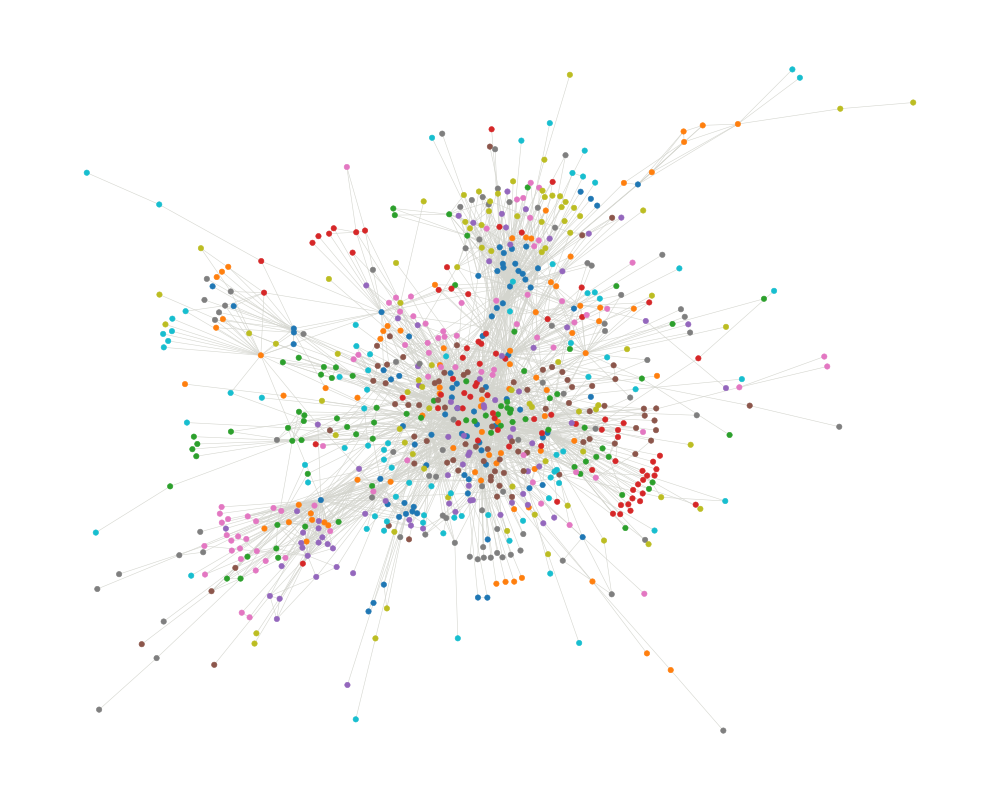
\includegraphics[width=0.9\textwidth]{Graphics/GOTPlot.png}
  \caption{Game of Thrones Graph 2.0, \\
  selbst erstellt}
  \label{fig:GOT2.0}
\end{figure}
\FloatBarrier

Dieser Plot bleibt absichtlich unkommentiert, da er lediglich zur Argumentation für die Verteilung der Zentralitäten benötigt wird und daher die visuelle Form des Graphen nur von zweitrangiger Bedeutung für diese Arbeit ist. Zudem ist zu vermerken, dass der eigentliche Datensatz gewichtet ist, und die bisher generierten Graph daher bereits schon visuell nicht dem Graphen aus Abbildung \ref{fig:GameOfThrones} ähnelt. Jedoch ist es sinnvoll die Gewichte außen vor zu lassen, da in dieser Arbeit ausschließlich ungewichtete Graphen nachgebildet, beziehungsweise behandelt werden. Nachdem die Daten im Generator eingelesen, die Zentralitäten berechnet und anschließend die Balkengraphen erstellt sind, ist folgender Plot \ref{fig:distributionGOT} zu sehen:

\FloatBarrier
\begin{figure}[h!]%
  \centering
   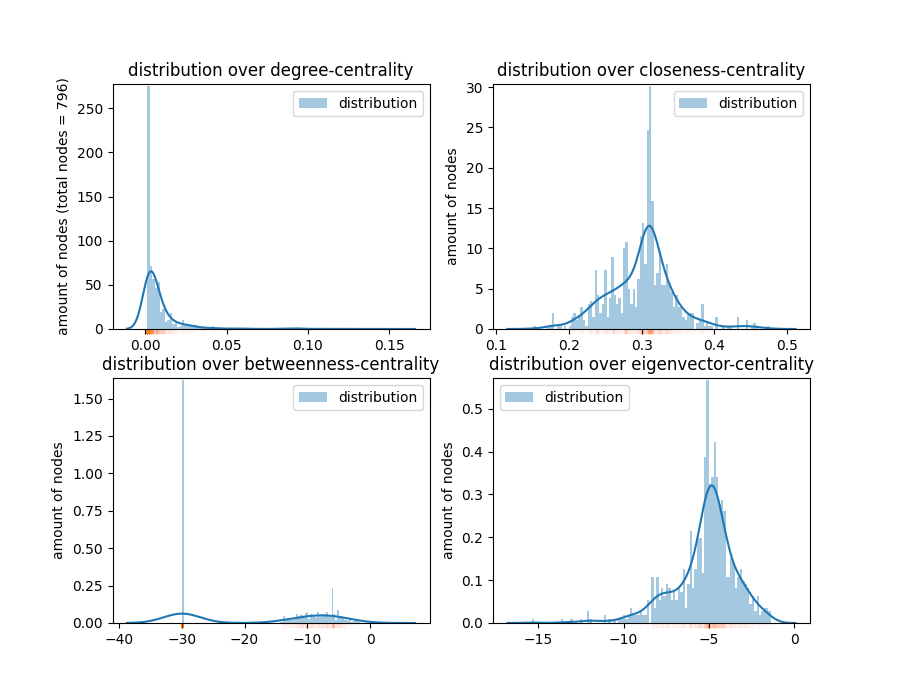
\includegraphics[width=0.7\textwidth]{Graphics/GOT-Distribution.png}
  \caption{Game of Thrones Verteilung der Zentralitäten}
  \label{fig:distributionGOT}
\end{figure}
\FloatBarrier
 
 Auf den ersten Blick wird bereits klar, die \textit{Zwischen-} und \textit{Eigenvektor-Zentralität} ähneln den Verteilungen in Abbildung \ref{fig:distributionALL} und es handelt sich um zwei annähernde \textit{Normal Verteilungen} also demnach \textit{Poisson-Verteilungen}. Beide Zentralitäten haben einen Ausschlag von mindestens einem Balken, was bereits im vorherigen Kapitel damit begründet wurde, dass es die Folge von vielen kürzesten Wegen ist, die stets über die gleichen
Knoten verlaufen, daher keine Alternativen im Graph existieren. \\

Die \textit{Grad-Zentralität} ähnelt einer Exponentialverteilung, welche ein Spezialfall der Poisson-Verteilung ist. Der Ausschlag der Balken ist erneut schnell erklärt. Es sind viele Knoten, in diesem Fall repräsentieren sie \textit{Game of Thrones} Charaktere, die alle gleich wichtig für den Graphen sind. Diese Knoten sind daher mit vielen anderen Knoten verbunden, werden also von vielen anderen Charakteren gekannt oder kennen viele andere Charaktere. Im Allgemeinen sind die Balkendiagramme der Zentralitäten aus Abbildung \ref{fig:distributionGOT} leider verglichen mit Abbildung \ref{fig:distributionALL} nicht zufriedenstellend, da sie sich untereinander nicht ähneln. Der Grund, warum die Ergebnisse stark abweicht ist vermutlich, dass es sich bei dem Graphen um fiktive Charaktere handelt. Dadurch kann es schnell zu Unstimmigkeiten kommen. Zudem war der Datensatz, bevor er im Zusammenhang dieser Arbeit verwendet wurde, gewichtet. Das kann durchaus zu anderen Werten bei der Berechnung der Zentralitäten führen. Doch wurde der Datensatz in dieser Arbeit ungewichtet betrachtet, um ihn besser mit den generierten Graphen zu vergleichen, welche ungewichtet sind. Dies kann einen Grund für Unstimmigkeiten darstellen. Zudem ist die Anzahl der geplotteten Balken stark erhöht und so fallen Unstimmigkeiten womöglich auch schneller auf. Doch wird erneut bei der Abbildung \ref{fig:distributionGOT} deutlich, dass die Zentralitäten, bis auf die Zwischen-Zentralität, tatsächlich annähernd als Poisson-Verteilung interpretiert werden können. Warum dies bei der Zwischen-Zentralität nicht der Fall ist, erscheint mir unschlüssig. \\ 

Dennoch soll die Theorie, dass Zentralitäten Poisson-Verteilt sind, nicht verworfen werden und wir betrachten noch einen weiteren Datensatz. Der nächste Datensatz, der aus \textit{Kreisen} (oder \textit{Freundeslisten}) besteht, ist von Facebook veröffentlicht worden \cite{FBData}. Die Daten wurden jedoch vor der Veröffentlichung von Facebook anonymisiert, daher ist lediglich bekannt, dass es sich bei dem Datensatz um politische Interessen handelt. So kann mit dem Datensatz feststellt werden, dass zwei Nutzer die gleiche politische Zugehörigkeit haben, aber nicht, was ihre individuelle politische Zugehörigkeit bedeutet \cite{FBData}.
Nachdem die Daten wieder in eine \textit{.CSV} Datei umgewandelt und anschließend geplottet wurden, ist folgenden Graphen entstanden: 


\FloatBarrier
\begin{figure}[h!]%
  \centering
 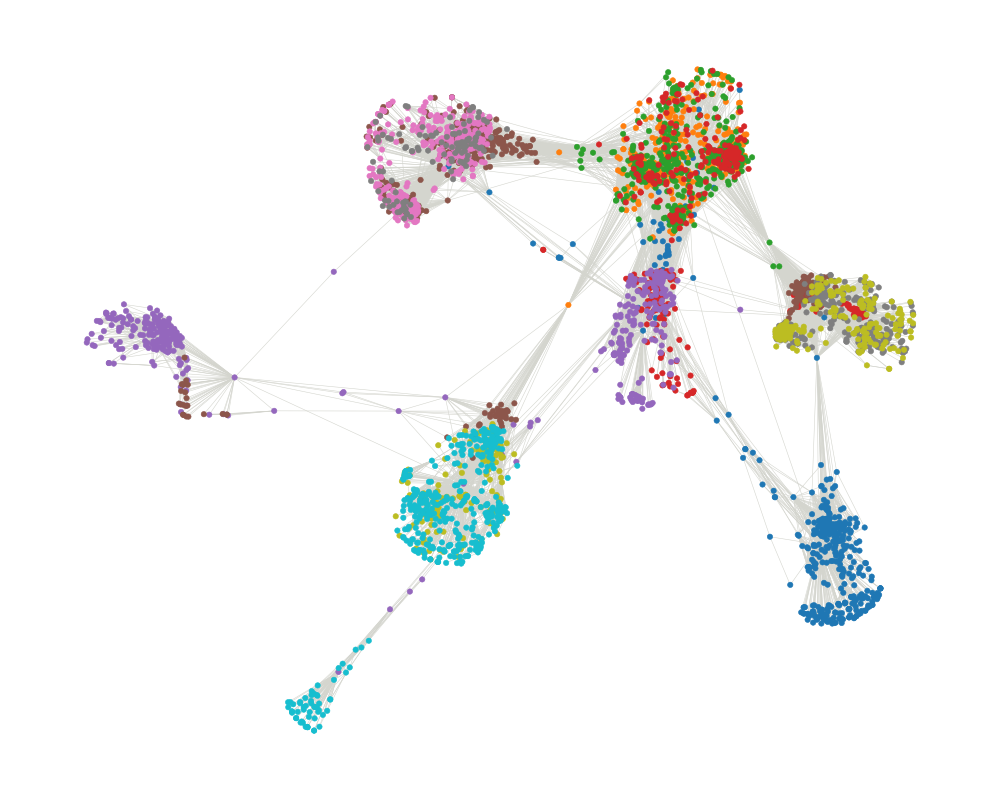
\includegraphics[width=0.9\textwidth]{Graphics/FacebookPoliticalPlot.png}
  \caption{Facebook Graph mit den Datensätzen aus \cite{FBData}}
  \label{fig:FacebookGraph}
\end{figure}
\FloatBarrier



Der Graph ähnelt auf den ersten Blick keinem, der bisher generierten Graphen. Zudem fällt aber sofort auf, dass dieser Graph aus deutlich mehr Knoten besteht, zudem weniger Subgraphen, beziehungsweise Cluster, besitzt aber dennoch eine grundsätzlich ähnliche Struktur zu unserem Graphen in Abbildung \ref{fig:SNA} aufweist. Nun interessiert uns jedoch, wie diese Zentralitäten verteilt sind und ob dieser Graph die erwarteten Verteilungen nachweist. Die Zentralitäten wurden erneut berechnet und es sich folgende Verteilungen entstanden:

\FloatBarrier
\begin{figure}[h!]%
  \centering
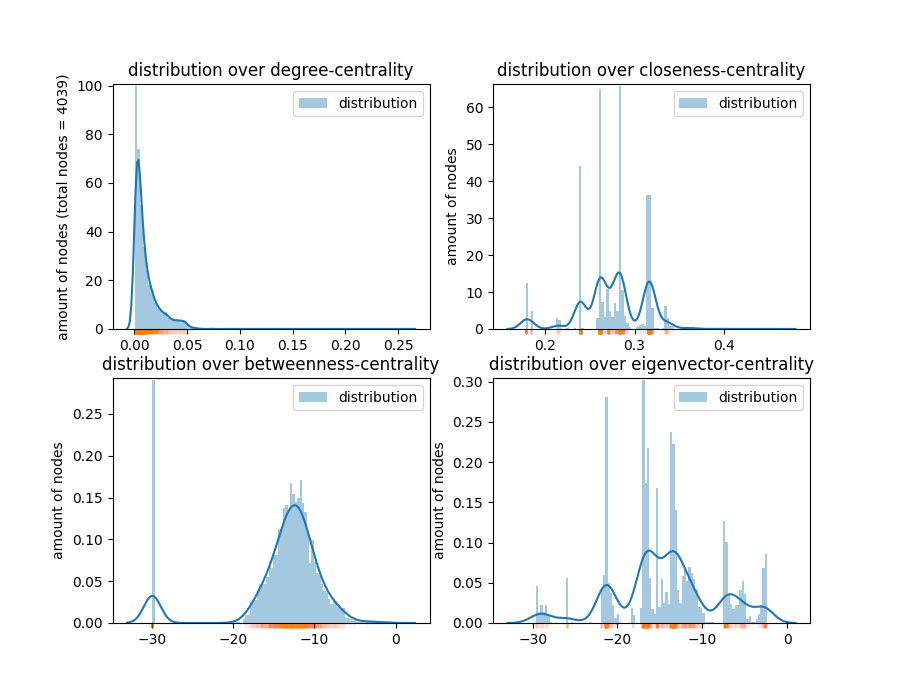
\includegraphics[width=0.7\textwidth]{Graphics/facebookLOG.png}
  \caption{Facebook Graph Distribution}
  \label{fig:FacebookGraphDistribution}
\end{figure}
\FloatBarrier

Die \textit{Grad-Zentralität} fällt hier direkt auf, denn es handelt sich erneut um eine Exponentialverteilung. Die anderen Balkendiagramme der \textit{Nähe-} und \textit{Eigenvektor-Zentralität} ähneln jedoch den Verteilungen aus Abbildung \ref{fig:distributionALL} keinesfalls. Was zudem auffällt ist, dass die Diagramme, bis auf die Verteilung der Zwischen-Zentralität, an die Verteilungen von Abbildung \ref{fig:distributionGOT} erinnern, welche im Endeffekt alle annähernd Poisson-Verteilt sind. Auch wenn diese Ergebnisse vielleicht ernüchternd sind, wollen wir uns überlegen, woran dies liegen kann. Bei der \textit{Nähe-} und \textit{Eigenvektor-Zentralität} ist eine starke Schwankung der Balken zu erkennen, wodurch mathematischen Wahrscheinlichkeitsverteilungen schwer erkennbar sind. Visuell fällt jedoch auf, dass der Graph in Abbildung \ref{fig:FacebookGraphDistribution} verglichen mit dem Plot des Graphen in Abbildung \ref{fig:SNA} durchaus Parallelen aufweist. Es sind deutliche Ansammlungen von Knoten erkennbar, die auch als Cluster bezeichnet werden können. Zwischen den Cluster sind, so wie bei Abbildung \ref{fig:SNA}, einige Kanten zu erkennen, die die Cluster untereinander verbinden. Natürlich weist der obige Graph in Abbildung \ref{fig:FacebookGraph} deutlich mehr Kanten und Knoten auf, als die bisherigen Graphen. Unsere Graphen haben im Schnitt um die \textbf{950} Knoten und \textbf{8700} Kanten, daher also circa neun mal so viele Kanten wie Knoten. Auch existieren im Schnitt um die \textbf{10100} Cliquen, welche maximal acht Knoten groß sind. Bei dem Facebook Graphen in Abbildung \ref{fig:FacebookGraph} hingegen \textbf{4093} Knoten und \textbf{88234} Kanten. Das heißt circa einundzwanzig mal so viele Kanten wie Knoten. Leider ist die Anzahl an Knoten und Kanten des Graphen in Abbildung \ref{fig:FacebookGraph} nur durch die Homepage \cite{FBData} bekannt, denn der Datensatz ist zu groß, um die Analyse der Zentralitäten und die Untersuchung auf Cliquen zu Ende zu führen. Daher ist auch die genaue Anzahl an Cliquen dieses Graphen unbekannt, doch kann vermutet werden, dass diese möglicherweise höher sind als bei Abbildung \ref{fig:distributionALL}, denn es existieren mehr Knoten mit ähnlich hohen Zentralitäten. \\

\newpage
Schließlich wird doch noch ein letzter Versuch gestartet, und die Kanten und Knoten im Code des Graphen Generators werden erhöht, um damit die selben Relation zu erhalten wie in Abbildung \ref{fig:FacebookGraph}. Dadurch wird womöglich gezeigt, dass alle vier untersuchten Zentralitäten annähernd Poisson verteilt sind. Es darf aber auf jeden Fall festgehalten werden, dass die \textit{Betweenness-} und \textit{Eigenvektor-Zentralität} bei allen untersuchten Datensätzen starke Parallelen zu den Verteilungen des generierten sozialen Netzwerk nachweisen. Jedoch ist nach wie vor die Verteilung der \textit{Grad-Zentralität} verwunderlich. Daher ist es ratsam, den Code und den damit verbundenen Plot so anzupassen, dass es Abbildung \ref{fig:FacebookGraphDistribution} ähnelt. Anschließend kann die Verteilungen der Zentralitäten betrachtet und dadurch womöglich eine genauere Aussage erzielt werden. 


\section{Anpassung des generierten sozialen Netzwerks}
Der folgende Plot wird nun weitestgehend an Abbildung \ref{fig:FacebookGraphDistribution} angepasst. An dieser Stelle muss betont werden, dass es sich bei den bisher generierten sozialen Netzwerken keinesfalls um untypische oder falsche soziale Netzwerke handelt, siehe Tabelle \ref{TableEigenschaften} und Tabelle \ref{TableEigenschaften2.0}. In diesem Abschnitt wird lediglich eine bessere Vergleichsbasis hergestellt. Dies wird ermöglicht, indem zum einen die Anzahl an Cluster auf \textbf{7} Stück anpasst und die Anzahl der Knoten pro Cluster erhöht wird. Gleichzeitig sollen die jeweiligen Größen deutlich mehr variieren und vor allem die Kanten-Menge, also Anzahl an Verbindungen, stark erhöht werden. Schließlich erhält man folgende Graphen \ref{fig:ourGraphFinalPlot}: 

\FloatBarrier
\begin{figure}[h!]%
  \centering
  \subfloat[][]{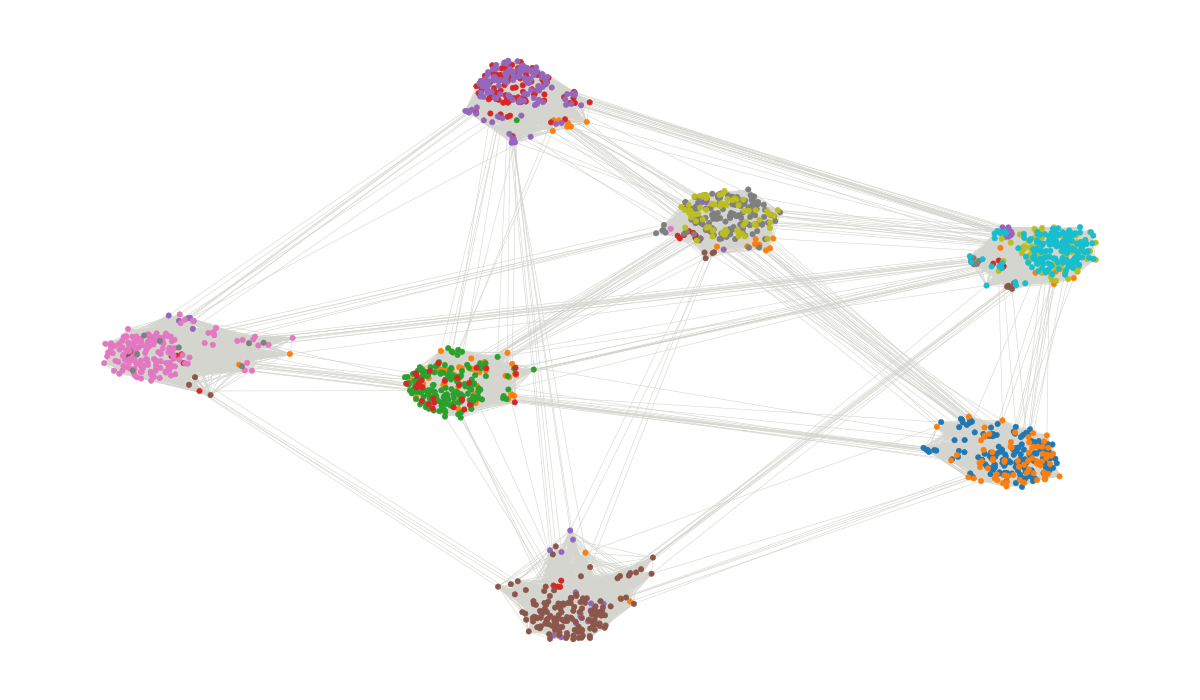
\includegraphics[width=0.7\textwidth]{Graphics/generatedPlotFinal.png}}%
  \qquad
  \subfloat[][]{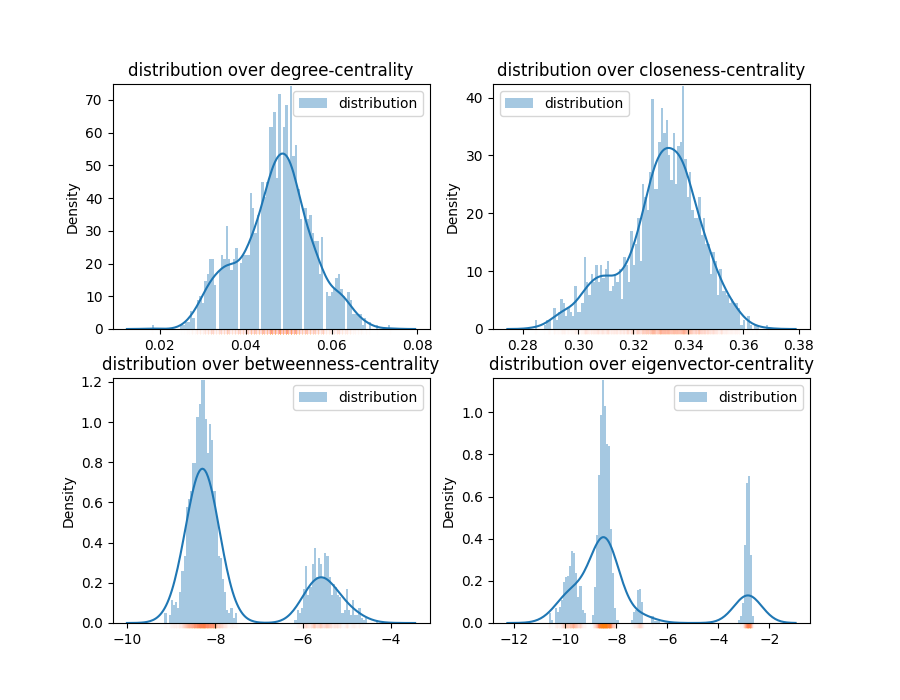
\includegraphics[width=0.6\textwidth]{Graphics/generatedPlotDensity.png}}
  \caption{Final optimierter Graph}
  \label{fig:ourGraphFinalPlot}
\end{figure}
\FloatBarrier

Es ist direkt ersichtlich, ohne die Werte genauer analysiert zu haben, dass kein zu Abbildung \ref{fig:FacebookGraphDistribution} identischer Graph, beziehungsweise Plot, erzeugt wurde. Allgemein sind aber die in dieser Arbeit generierten Graphen, auch wenn die Varianz der Graph-Größen best möglichst garantiert wird, auf den ersten Blick visuell gesehen ähnlich groß. Positiv zu erwähnen ist, dass bei der Verteilung der \textit{Zwischen-} und \textit{Eigenvektor-Zentralität} eine absolute Verbesserung erzielt, indem die Zentralitäten, bevor sie geplottet werden, logarithmiert werden. Dies wurde nachträglich auch bei allen vorherigen Verteilungen gemacht. Das ermöglicht es, die Verteilung auseinander zu zerren, da sich die Werte davor stets um \textbf{0.0} verteilt haben. Nun fällt auf, dass die Verteilungen mancher Zentralitäten doch sehr ähnlich sind. Die Verteilung der \textit{Grad-} und \textit{Nähe-Zentralität} erinnert beispielsweise wieder an eine Normalverteilung, welche wieder die Bedingung der Poisson-Verteilung aus Tabelle \ref{TableEigenschaften2.0} erfüllt. Auch die \textit{Zwischen-} und \textit{Eigenvektor-Zentralität} weisen Parallelen auf, denn sie sehen wie jeweils zwei zusammengefügte Normalverteilungen aus. Erneut können diese als annähernde Poisson-Verteilung gesehen werden. Das heißt, die Abbildung \ref{fig:ourGraphFinalPlot} erfüllt die Eigenschaft aus Tabelle \ref{TableEigenschaften2.0} und visuell betrachtet auch die Eigenschaften aus Tabelle \ref{TableEigenschaften}. Im Allgemeinen kann also gesagt werden, dass es sich um ein typisches soziales Netzwerk handelt. \\

Zwar entsprechen die Verteilungen von Abbildung \ref{fig:ourGraphFinalPlot} nicht den Verteilungen von \ref{fig:FacebookGraphDistribution}, doch hat die Verbesserung des Graphen in diesem Kapitel dennoch viel gebracht. Unter anderem konnte bewiesen werden, dass mit wenigen Anpassungen des Codes, annähernd vergleichbare Verteilungen erhalten werden. Außerdem wurde auf diese Weise eine Abbildung \ref{fig:ourGraphFinalPlot} generiert, die visuell betrachtet durchaus der Abbildung \ref{fig:FacebookGraph} ähnelt. Um jedoch den idealen Vergleich herzustellen zu können, müssten größere Änderungen am Code vorgenommen werden. Das entspricht jedoch nicht mehr dem Umfang dieser Arbeit und wird daher nicht weiter fortgeführt. Jedoch kann als Fazit festgehalten werden, dass auch wenn die Verteilungen untereinander nicht perfekte Ähnlichkeiten aufweisen, sie im Endeffekt dennoch typische soziale Netzwerke sind und weitestgehend die Anforderungen aus Tabelle \ref{TableEigenschaften} und Tabelle \ref{TableEigenschaften2.0} erfüllen. 



